\documentclass[11pt,a4paper]{article}
\usepackage[utf8]{inputenc}

\usepackage{geometry}
 \geometry{
 left=25mm,
 top=25mm,
 right=25mm,
 bottom=25mm,
 }
\usepackage{graphicx}
\usepackage{bm}
\usepackage{url}
\usepackage{amsmath}
\usepackage{tikz}
\usepackage{todonotes}
%\renewcommand{\baselinestretch}{1.25}

\title{Decoding Performance of Convolutional Codes}
\author{Rasmus Vestergaard, Stefan Bejan and Daniel Pytlos}
\date{March 2017}

\begin{document}
\maketitle
\todo[inline] {Compare different codes with the same constraint length but different (same number of) generator polynomials in both burst-error and random-error correction.}
\todo[inline] {Compare different codes with the same constraint length and different code rate (more generator polynomials).}
\todo[inline] {Create a markov burst-error channel?}
\begin{figure} [h]
\centering
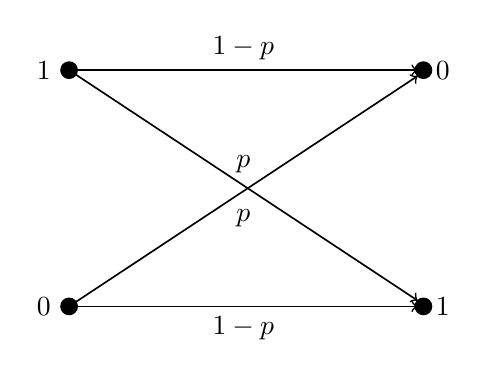
\begin{tikzpicture}
\centering
\filldraw (0,0) circle (3pt);
\filldraw (0,3) circle (3pt);
\filldraw (4.5,0) circle (3pt);
\filldraw (4.5,3) circle (3pt);
\draw[->,line width=0.6pt] (0,3) node[left=3pt] {$1$} -- node[above=1pt] {$p$} (4.425,0.075);
\draw[->,line width=0.6pt] (0,0) node[left=3pt] {$0$} -- node[below=3pt] {$p$} (4.425,2.925);
\draw[->,line width=0.6pt] (0,0) -- node[below] {$1-p$} (4.425,0.00)  node[right=3pt] {$1$};
\draw[->,line width=0.6pt] (0,3) -- node[above] {$1-p$} (4.425,3) node[right=3pt] {$0$};
\end{tikzpicture}
\caption{Binary Symmetric Channel\label{fig:bscChannel}}
\end{figure}
\end{document}